\documentclass[border=12pt]{standalone}

\usepackage{tikz}
\usetikzlibrary{arrows.meta,positioning,fit,calc}

\definecolor{embcol}{RGB}{219,234,254}
\definecolor{attncol}{RGB}{254,215,170}
\definecolor{maskcol}{RGB}{233,213,255}
\definecolor{crosscol}{RGB}{187,247,208}
\definecolor{ffcol}{RGB}{199,210,254}
\definecolor{normcol}{RGB}{254,240,138}
\definecolor{lincol}{RGB}{226,232,240}
\definecolor{softcol}{RGB}{254,205,211}
\definecolor{bordercol}{RGB}{71,85,105}
\definecolor{linecol}{RGB}{51,65,85}
\definecolor{rescol}{RGB}{120,113,108}
\definecolor{kvcol}{RGB}{4,120,87}
\definecolor{stackcol}{RGB}{148,163,184}
\definecolor{labelcol}{RGB}{30,41,59}

\begin{document}
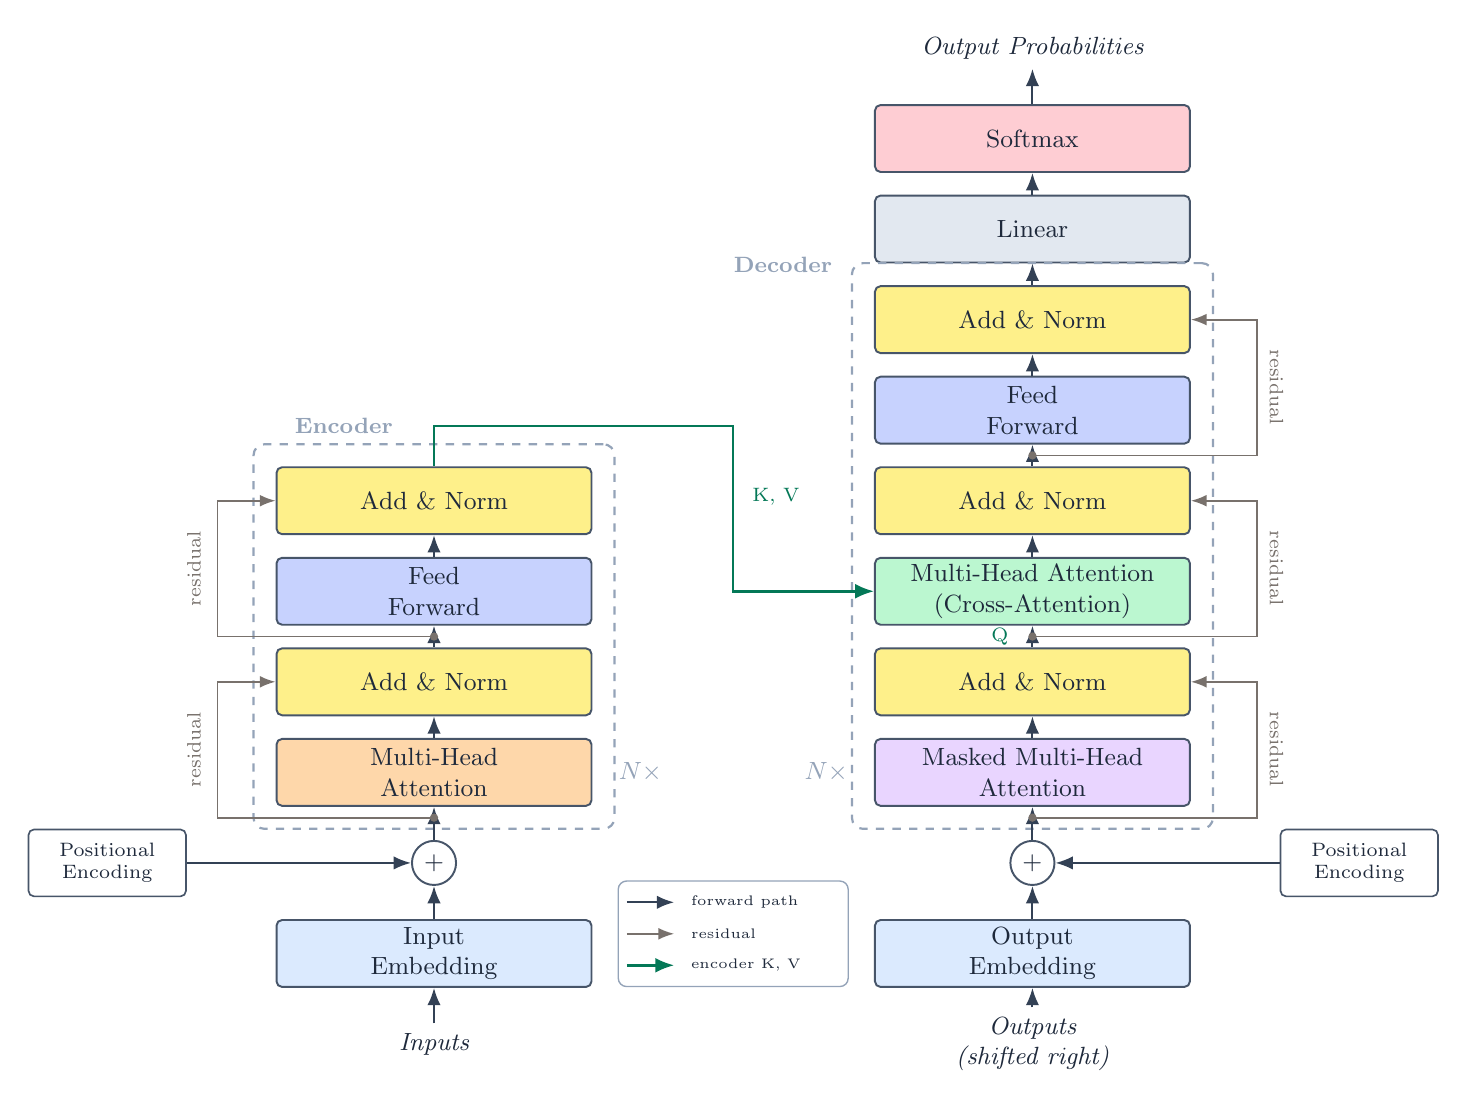
\begin{tikzpicture}[
  x=1cm, y=1cm,
  block/.style={
    draw=bordercol, line width=0.7pt, rounded corners=2pt,
    minimum width=4.0cm, minimum height=0.85cm,
    align=center, font=\small, text=labelcol, inner sep=2pt
  },
  plus/.style={
    draw=bordercol, line width=0.7pt, circle, minimum size=0.56cm,
    inner sep=0pt, font=\small, text=labelcol, fill=white
  },
  side/.style={
    draw=bordercol, line width=0.6pt, rounded corners=2pt, fill=white,
    minimum width=2.0cm, minimum height=0.85cm,
    align=center, font=\scriptsize, text=labelcol, inner sep=2pt
  },
  io/.style={font=\small\itshape, text=labelcol, align=center},
  flow/.style={draw=linecol, line width=0.75pt, -{Latex[length=2.2mm,width=1.7mm]}},
  res/.style={draw=rescol, line width=0.65pt, -{Latex[length=2.0mm,width=1.5mm]}},
  kv/.style={draw=kvcol, line width=0.9pt, -{Latex[length=2.4mm,width=1.9mm]}},
  tag/.style={font=\scriptsize, text=rescol},
  stackbox/.style={draw=stackcol, line width=0.8pt, dashed, rounded corners=4pt, inner sep=0.28cm}
]

%% ===================== Encoder stack (left) =====================
\node[io]                    (ein)  at (0,-0.60) {Inputs};
\node[block, fill=embcol]    (eemb) at (0, 0.55) {Input\\Embedding};
\node[plus]                  (epls) at (0, 1.70) {$+$};
\node[block, fill=attncol]   (emha) at (0, 2.85) {Multi-Head\\Attention};
\node[block, fill=normcol]   (ean1) at (0, 4.00) {Add \& Norm};
\node[block, fill=ffcol]     (eff)  at (0, 5.15) {Feed\\Forward};
\node[block, fill=normcol]   (ean2) at (0, 6.30) {Add \& Norm};
\node[side]                  (epe)  at (-4.15, 1.70) {Positional\\Encoding};

%% ===================== Decoder stack (right) ====================
\node[io]                    (din)  at (7.6,-0.60) {Outputs\\(shifted right)};
\node[block, fill=embcol]    (demb) at (7.6, 0.55) {Output\\Embedding};
\node[plus]                  (dpls) at (7.6, 1.70) {$+$};
\node[block, fill=maskcol]   (dmha) at (7.6, 2.85) {Masked Multi-Head\\Attention};
\node[block, fill=normcol]   (dan1) at (7.6, 4.00) {Add \& Norm};
\node[block, fill=crosscol]  (dxa)  at (7.6, 5.15) {Multi-Head Attention\\(Cross-Attention)};
\node[block, fill=normcol]   (dan2) at (7.6, 6.30) {Add \& Norm};
\node[block, fill=ffcol]     (dff)  at (7.6, 7.45) {Feed\\Forward};
\node[block, fill=normcol]   (dan3) at (7.6, 8.60) {Add \& Norm};
\node[block, fill=lincol]    (dlin) at (7.6, 9.75) {Linear};
\node[block, fill=softcol]   (dsm)  at (7.6,10.90) {Softmax};
\node[io]                    (dout) at (7.6,12.05) {Output Probabilities};
\node[side]                  (dpe)  at (11.75, 1.70) {Positional\\Encoding};

%% ===================== N x stack frames =========================
\node[stackbox, fit=(emha)(ean2)] (encframe) {};
\node[stackbox, fit=(dmha)(dan3)] (decframe) {};
\node[font=\small, text=stackcol] at (2.62, 2.85) {$N\times$};
\node[font=\small, text=stackcol] at (4.98, 2.85) {$N\times$};
\node[font=\footnotesize\bfseries, text=stackcol, anchor=east] at (-0.40, 7.25) {Encoder};
\node[font=\footnotesize\bfseries, text=stackcol, anchor=east] at ( 5.18, 9.30) {Decoder};

%% ===================== Main flow: encoder =======================
\draw[flow] (ein)  -- (eemb);
\draw[flow] (eemb) -- (epls);
\draw[flow] (epls) -- (emha);
\draw[flow] (emha) -- (ean1);
\draw[flow] (ean1) -- (eff);
\draw[flow] (eff)  -- (ean2);
\draw[flow] (epe)  -- (epls);

%% ===================== Main flow: decoder =======================
\draw[flow] (din)  -- (demb);
\draw[flow] (demb) -- (dpls);
\draw[flow] (dpls) -- (dmha);
\draw[flow] (dmha) -- (dan1);
\draw[flow] (dan1) -- (dxa);
\draw[flow] (dxa)  -- (dan2);
\draw[flow] (dan2) -- (dff);
\draw[flow] (dff)  -- (dan3);
\draw[flow] (dan3) -- (dlin);
\draw[flow] (dlin) -- (dsm);
\draw[flow] (dsm)  -- (dout);
\draw[flow] (dpe)  -- (dpls);
\node[font=\scriptsize, text=kvcol, anchor=east] at (7.42, 4.575) {Q};

%% ===================== Residual connections =====================
% encoder: self-attention sublayer
\draw[res] (0,2.275) -- (-2.75,2.275) -- (-2.75,4.00) -- (ean1.west);
% encoder: feed-forward sublayer
\draw[res] (0,4.575) -- (-2.75,4.575) -- (-2.75,6.30) -- (ean2.west);
% decoder: masked self-attention sublayer
\draw[res] (7.6,2.275) -- (10.45,2.275) -- (10.45,4.00) -- (dan1.east);
% decoder: cross-attention sublayer
\draw[res] (7.6,4.575) -- (10.45,4.575) -- (10.45,6.30) -- (dan2.east);
% decoder: feed-forward sublayer
\draw[res] (7.6,6.875) -- (10.45,6.875) -- (10.45,8.60) -- (dan3.east);

\fill[rescol] (0,2.275) circle (1.5pt);
\fill[rescol] (0,4.575) circle (1.5pt);
\fill[rescol] (7.6,2.275) circle (1.5pt);
\fill[rescol] (7.6,4.575) circle (1.5pt);
\fill[rescol] (7.6,6.875) circle (1.5pt);

\node[tag, rotate=90]  at (-3.05, 3.14) {residual};
\node[tag, rotate=90]  at (-3.05, 5.44) {residual};
\node[tag, rotate=-90] at (10.70, 3.14) {residual};
\node[tag, rotate=-90] at (10.70, 5.44) {residual};
\node[tag, rotate=-90] at (10.70, 7.74) {residual};

%% ============ Encoder output -> decoder cross-attention =========
\draw[kv] (ean2.north) -- (0,7.25) -- (3.80,7.25) -- (3.80,5.15) -- (dxa.west);
\node[font=\scriptsize, text=kvcol, anchor=west] at (3.92, 6.35) {K, V};

%% ===================== Legend ===================================
\draw[draw=stackcol, line width=0.5pt, rounded corners=3pt, fill=white]
      (2.34,0.13) rectangle (5.26,1.47);
\draw[flow] (2.45,1.20) -- (3.05,1.20);
\node[font=\tiny, text=labelcol, anchor=west] at (3.14,1.20) {forward path};
\draw[res]  (2.45,0.80) -- (3.05,0.80);
\node[font=\tiny, text=labelcol, anchor=west] at (3.14,0.80) {residual};
\draw[kv]   (2.45,0.40) -- (3.05,0.40);
\node[font=\tiny, text=labelcol, anchor=west] at (3.14,0.40) {encoder K, V};

\end{tikzpicture}
\end{document}
